
%% bare_conf.tex
%% V1.3
%% 2007/01/11
%% by Michael Shell
%% See:
%% http://www.michaelshell.org/
%% for current contact information.
%%
%% This is a skeleton file demonstrating the use of IEEEtran.cls
%% (requires IEEEtran.cls version 1.7 or later) with an IEEE conference paper.
%%
%% Support sites:
%% http://www.michaelshell.org/tex/ieeetran/
%% http://www.ctan.org/tex-archive/macros/latex/contrib/IEEEtran/
%% and
%% http://www.ieee.org/

%%*************************************************************************
%% Legal Notice:
%% This code is offered as-is without any warranty either expressed or
%% implied; without even the implied warranty of MERCHANTABILITY or
%% FITNESS FOR A PARTICULAR PURPOSE! 
%% User assumes all risk.
%% In no event shall IEEE or any contributor to this code be liable for
%% any damages or losses, including, but not limited to, incidental,
%% consequential, or any other damages, resulting from the use or misuse
%% of any information contained here.
%%
%% All comments are the opinions of their respective authors and are not
%% necessarily endorsed by the IEEE.
%%
%% This work is distributed under the LaTeX Project Public License (LPPL)
%% ( http://www.latex-project.org/ ) version 1.3, and may be freely used,
%% distributed and modified. A copy of the LPPL, version 1.3, is included
%% in the base LaTeX documentation of all distributions of LaTeX released
%% 2003/12/01 or later.
%% Retain all contribution notices and credits.
%% ** Modified files should be clearly indicated as such, including  **
%% ** renaming them and changing author support contact information. **
%%
%% File list of work: IEEEtran.cls, IEEEtran_HOWTO.pdf, bare_adv.tex,
%%                    bare_conf.tex, bare_jrnl.tex, bare_jrnl_compsoc.tex
%%*************************************************************************

% *** Authors should verify (and, if needed, correct) their LaTeX system  ***
% *** with the testflow diagnostic prior to trusting their LaTeX platform ***
% *** with production work. IEEE's font choices can trigger bugs that do  ***
% *** not appear when using other class files.                            ***
% The testflow support page is at:
% http://www.michaelshell.org/tex/testflow/



% Note that the a4paper option is mainly intended so that authors in
% countries using A4 can easily print to A4 and see how their papers will
% look in print - the typesetting of the document will not typically be
% affected with changes in paper size (but the bottom and side margins will).
% Use the testflow package mentioned above to verify correct handling of
% both paper sizes by the user's LaTeX system.
%
% Also note that the "draftcls" or "draftclsnofoot", not "draft", option
% should be used if it is desired that the figures are to be displayed in
% draft mode.
%
\documentclass[conference]{IEEEtran}
% Add the compsoc option for Computer Society conferences.
%
% If IEEEtran.cls has not been installed into the LaTeX system files,
% manually specify the path to it like:
% \documentclass[conference]{../sty/IEEEtran}




% Some very useful LaTeX packages include:
% (uncomment the ones you want to load)


% *** MISC UTILITY PACKAGES ***
%
%\usepackage{ifpdf}
% Heiko Oberdiek's ifpdf.sty is very useful if you need conditional
% compilation based on whether the output is pdf or dvi.
% usage:
% \ifpdf
%   % pdf code
% \else
%   % dvi code
% \fi
% The latest version of ifpdf.sty can be obtained from:
% http://www.ctan.org/tex-archive/macros/latex/contrib/oberdiek/
% Also, note that IEEEtran.cls V1.7 and later provides a builtin
% \ifCLASSINFOpdf conditional that works the same way.
% When switching from latex to pdflatex and vice-versa, the compiler may
% have to be run twice to clear warning/error messages.
\usepackage{graphicx}





% *** CITATION PACKAGES ***
%
%\usepackage{cite}
% cite.sty was written by Donald Arseneau
% V1.6 and later of IEEEtran pre-defines the format of the cite.sty package
% \cite{} output to follow that of IEEE. Loading the cite package will
% result in citation numbers being automatically sorted and properly
% "compressed/ranged". e.g., [1], [9], [2], [7], [5], [6] without using
% cite.sty will become [1], [2], [5]--[7], [9] using cite.sty. cite.sty's
% \cite will automatically add leading space, if needed. Use cite.sty's
% noadjust option (cite.sty V3.8 and later) if you want to turn this off.
% cite.sty is already installed on most LaTeX systems. Be sure and use
% version 4.0 (2003-05-27) and later if using hyperref.sty. cite.sty does
% not currently provide for hyperlinked citations.
% The latest version can be obtained at:
% http://www.ctan.org/tex-archive/macros/latex/contrib/cite/
% The documentation is contained in the cite.sty file itself.






% *** GRAPHICS RELATED PACKAGES ***
%
\ifCLASSINFOpdf
  % \usepackage[pdftex]{graphicx}
  % declare the path(s) where your graphic files are
  % \graphicspath{{../pdf/}{../jpeg/}}
  % and their extensions so you won't have to specify these with
  % every instance of \includegraphics
  % \DeclareGraphicsExtensions{.pdf,.jpeg,.png}
\else
  % or other class option (dvipsone, dvipdf, if not using dvips). graphicx
  % will default to the driver specified in the system graphics.cfg if no
  % driver is specified.
  % \usepackage[dvips]{graphicx}
  % declare the path(s) where your graphic files are
  % \graphicspath{{../eps/}}
  % and their extensions so you won't have to specify these with
  % every instance of \includegraphics
  % \DeclareGraphicsExtensions{.eps}
\fi
% graphicx was written by David Carlisle and Sebastian Rahtz. It is
% required if you want graphics, photos, etc. graphicx.sty is already
% installed on most LaTeX systems. The latest version and documentation can
% be obtained at: 
% http://www.ctan.org/tex-archive/macros/latex/required/graphics/
% Another good source of documentation is "Using Imported Graphics in
% LaTeX2e" by Keith Reckdahl which can be found as epslatex.ps or
% epslatex.pdf at: http://www.ctan.org/tex-archive/info/
%
% latex, and pdflatex in dvi mode, support graphics in encapsulated
% postscript (.eps) format. pdflatex in pdf mode supports graphics
% in .pdf, .jpeg, .png and .mps (metapost) formats. Users should ensure
% that all non-photo figures use a vector format (.eps, .pdf, .mps) and
% not a bitmapped formats (.jpeg, .png). IEEE frowns on bitmapped formats
% which can result in "jaggedy"/blurry rendering of lines and letters as
% well as large increases in file sizes.
%
% You can find documentation about the pdfTeX application at:
% http://www.tug.org/applications/pdftex





% *** MATH PACKAGES ***
%
%\usepackage[cmex10]{amsmath}
% A popular package from the American Mathematical Society that provides
% many useful and powerful commands for dealing with mathematics. If using
% it, be sure to load this package with the cmex10 option to ensure that
% only type 1 fonts will utilized at all point sizes. Without this option,
% it is possible that some math symbols, particularly those within
% footnotes, will be rendered in bitmap form which will result in a
% document that can not be IEEE Xplore compliant!
%
% Also, note that the amsmath package sets \interdisplaylinepenalty to 10000
% thus preventing page breaks from occurring within multiline equations. Use:
%\interdisplaylinepenalty=2500
% after loading amsmath to restore such page breaks as IEEEtran.cls normally
% does. amsmath.sty is already installed on most LaTeX systems. The latest
% version and documentation can be obtained at:
% http://www.ctan.org/tex-archive/macros/latex/required/amslatex/math/





% *** SPECIALIZED LIST PACKAGES ***
%
%\usepackage{algorithmic}
% algorithmic.sty was written by Peter Williams and Rogerio Brito.
% This package provides an algorithmic environment fo describing algorithms.
% You can use the algorithmic environment in-text or within a figure
% environment to provide for a floating algorithm. Do NOT use the algorithm
% floating environment provided by algorithm.sty (by the same authors) or
% algorithm2e.sty (by Christophe Fiorio) as IEEE does not use dedicated
% algorithm float types and packages that provide these will not provide
% correct IEEE style captions. The latest version and documentation of
% algorithmic.sty can be obtained at:
% http://www.ctan.org/tex-archive/macros/latex/contrib/algorithms/
% There is also a support site at:
% http://algorithms.berlios.de/index.html
% Also of interest may be the (relatively newer and more customizable)
% algorithmicx.sty package by Szasz Janos:
% http://www.ctan.org/tex-archive/macros/latex/contrib/algorithmicx/




% *** ALIGNMENT PACKAGES ***
%
%\usepackage{array}
% Frank Mittelbach's and David Carlisle's array.sty patches and improves
% the standard LaTeX2e array and tabular environments to provide better
% appearance and additional user controls. As the default LaTeX2e table
% generation code is lacking to the point of almost being broken with
% respect to the quality of the end results, all users are strongly
% advised to use an enhanced (at the very least that provided by array.sty)
% set of table tools. array.sty is already installed on most systems. The
% latest version and documentation can be obtained at:
% http://www.ctan.org/tex-archive/macros/latex/required/tools/


%\usepackage{mdwmath}
%\usepackage{mdwtab}
% Also highly recommended is Mark Wooding's extremely powerful MDW tools,
% especially mdwmath.sty and mdwtab.sty which are used to format equations
% and tables, respectively. The MDWtools set is already installed on most
% LaTeX systems. The lastest version and documentation is available at:
% http://www.ctan.org/tex-archive/macros/latex/contrib/mdwtools/


% IEEEtran contains the IEEEeqnarray family of commands that can be used to
% generate multiline equations as well as matrices, tables, etc., of high
% quality.


%\usepackage{eqparbox}
% Also of notable interest is Scott Pakin's eqparbox package for creating
% (automatically sized) equal width boxes - aka "natural width parboxes".
% Available at:
% http://www.ctan.org/tex-archive/macros/latex/contrib/eqparbox/





% *** SUBFIGURE PACKAGES ***
%\usepackage[tight,footnotesize]{subfigure}
% subfigure.sty was written by Steven Douglas Cochran. This package makes it
% easy to put subfigures in your figures. e.g., "Figure 1a and 1b". For IEEE
% work, it is a good idea to load it with the tight package option to reduce
% the amount of white space around the subfigures. subfigure.sty is already
% installed on most LaTeX systems. The latest version and documentation can
% be obtained at:
% http://www.ctan.org/tex-archive/obsolete/macros/latex/contrib/subfigure/
% subfigure.sty has been superceeded by subfig.sty.



%\usepackage[caption=false]{caption}
%\usepackage[font=footnotesize]{subfig}
% subfig.sty, also written by Steven Douglas Cochran, is the modern
% replacement for subfigure.sty. However, subfig.sty requires and
% automatically loads Axel Sommerfeldt's caption.sty which will override
% IEEEtran.cls handling of captions and this will result in nonIEEE style
% figure/table captions. To prevent this problem, be sure and preload
% caption.sty with its "caption=false" package option. This is will preserve
% IEEEtran.cls handing of captions. Version 1.3 (2005/06/28) and later 
% (recommended due to many improvements over 1.2) of subfig.sty supports
% the caption=false option directly:
%\usepackage[caption=false,font=footnotesize]{subfig}
%
% The latest version and documentation can be obtained at:
% http://www.ctan.org/tex-archive/macros/latex/contrib/subfig/
% The latest version and documentation of caption.sty can be obtained at:
% http://www.ctan.org/tex-archive/macros/latex/contrib/caption/




% *** FLOAT PACKAGES ***
%
%\usepackage{fixltx2e}
% fixltx2e, the successor to the earlier fix2col.sty, was written by
% Frank Mittelbach and David Carlisle. This package corrects a few problems
% in the LaTeX2e kernel, the most notable of which is that in current
% LaTeX2e releases, the ordering of single and double column floats is not
% guaranteed to be preserved. Thus, an unpatched LaTeX2e can allow a
% single column figure to be placed prior to an earlier double column
% figure. The latest version and documentation can be found at:
% http://www.ctan.org/tex-archive/macros/latex/base/



%\usepackage{stfloats}
% stfloats.sty was written by Sigitas Tolusis. This package gives LaTeX2e
% the ability to do double column floats at the bottom of the page as well
% as the top. (e.g., "\begin{figure*}[!b]" is not normally possible in
% LaTeX2e). It also provides a command:
%\fnbelowfloat
% to enable the placement of footnotes below bottom floats (the standard
% LaTeX2e kernel puts them above bottom floats). This is an invasive package
% which rewrites many portions of the LaTeX2e float routines. It may not work
% with other packages that modify the LaTeX2e float routines. The latest
% version and documentation can be obtained at:
% http://www.ctan.org/tex-archive/macros/latex/contrib/sttools/
% Documentation is contained in the stfloats.sty comments as well as in the
% presfull.pdf file. Do not use the stfloats baselinefloat ability as IEEE
% does not allow \baselineskip to stretch. Authors submitting work to the
% IEEE should note that IEEE rarely uses double column equations and
% that authors should try to avoid such use. Do not be tempted to use the
% cuted.sty or midfloat.sty packages (also by Sigitas Tolusis) as IEEE does
% not format its papers in such ways.





% *** PDF, URL AND HYPERLINK PACKAGES ***
%
\usepackage[bookmarks=false]{hyperref}
\usepackage{breakurl}
% url.sty was written by Donald Arseneau. It provides better support for
% handling and breaking URLs. url.sty is already installed on most LaTeX
% systems. The latest version can be obtained at:
% http://www.ctan.org/tex-archive/macros/latex/contrib/misc/
% Read the url.sty source comments for usage information. Basically,
% \url{my_url_here}.





% *** Do not adjust lengths that control margins, column widths, etc. ***
% *** Do not use packages that alter fonts (such as pslatex).         ***
% There should be no need to do such things with IEEEtran.cls V1.6 and later.
% (Unless specifically asked to do so by the journal or conference you plan
% to submit to, of course. )


% correct bad hyphenation here
\hyphenation{op-tical net-works semi-conduc-tor}


\begin{document}
%
% paper title
% can use linebreaks \\ within to get better formatting as desired
\title{Are you being served: A Framework to manage Cloud outage repair times for Small Medium Enterprises.}


% author names and affiliations
%use a multiple column layout for up to three different
% affiliations
\author{\IEEEauthorblockN{Jonathan Dunne}
\IEEEauthorblockA{Hamilton Institute\\
Maynooth University\\\
Email: jonathan.dunne.2015@mumail.com}
\and
\IEEEauthorblockN{David Malone}
\IEEEauthorblockA{Hamilton Institute\\
Maynooth University\\
Email: david.malone@nuim.ie}}


% conference papers do not typically use \thanks and this command
% is locked out in conference mode. If really needed, such as for
% the acknowledgment of grants, issue a \IEEEoverridecommandlockouts
% after \documentclass

% for over three affiliations, or if they all won't fit within the width
% of the page, use this alternative format:
% 
%\author{\IEEEauthorblockN{Michael Shell\IEEEauthorrefmark{1},
%Homer Simpson\IEEEauthorrefmark{2},
%James Kirk\IEEEauthorrefmark{3}, 
%Montgomery Scott\IEEEauthorrefmark{3} and
%Eldon Tyrell\IEEEauthorrefmark{4}}
%\IEEEauthorblockA{\IEEEauthorrefmark{1}School of Electrical and Computer Engineering\\
%Georgia Institute of Technology,
%Atlanta, Georgia 30332--0250\\ Email: see http://www.michaelshell.org/contact.html}
%\IEEEauthorblockA{\IEEEauthorrefmark{2}Twentieth Century Fox, Springfield, USA\\
%Email: homer@thesimpsons.com}
%\IEEEauthorblockA{\IEEEauthorrefmark{3}Starfleet Academy, San Francisco, California 96678-2391\\
%Telephone: (800) 555--1212, Fax: (888) 555--1212}
%\IEEEauthorblockA{\IEEEauthorrefmark{4}Tyrell Inc., 123 Replicant Street, Los Angeles, California 90210--4321}}




% use for special paper notices
%\IEEEspecialpapernotice{(Invited Paper)}




% make the title area
\maketitle


\begin{abstract}
%\boldmath

Hosting software applications in a Cloud based infrastructure represents challenges for Small Medium Enterprises (SMEs), due to the variety of ways in which production outages can occur. We consider repair times for outage events in a framework where these downtimes are used to re-focus Systems Operations resources. Using an enterprise dataset, we address the question of how outage events are distributed and what relationship these events have with different types of failures that can occur in a cloud data centre. The proposed framework can aid SMEs to maintain a highly available On-Demand service infrastructure, with limited resources.
\end{abstract}
% IEEEtran.cls defaults to using nonbold math in the Abstract.
% This preserves the distinction between vectors and scalars. However,
% if the conference you are submitting to favors bold math in the abstract,
% then you can use LaTeX's standard command \boldmath at the very start
% of the abstract to achieve this. Many IEEE journals/conferences frown on
% math in the abstract anyway.

% no keywords

% For peer review papers, you can put extra information on the cover
% page as needed:
% \ifCLASSOPTIONpeerreview
% \begin{center} \bfseries EDICS Category: 3-BBND \end{center}
% \fi
%
% For peerreview papers, this IEEEtran command inserts a page break and
% creates the second title. It will be ignored for other modes.
\IEEEpeerreviewmaketitle

\section{Introduction}
% no \IEEEPARstart

SMEs have seen significant growth in recent years; a 71\% increase in employment (excluding financial sector) was recorded in 2014. Moreover SMEs employed almost 90 million people in Europe. \cite{europa2015sme}. As the European economy continues to recover, both businesses and clients are looking for new avenues to drive growth across the EU and beyond. \par

One way to provide services with an elevated market reach is through a Software as a Service (SaaS) model. This cloud-based approach is seen as a shift away from highly complex bespoke solutions, to more focused and cost effective solutions \cite{cloudbook2015}. As customers demand highly effective services to solve their business problems, a cloud platform can help keep pace with these needs. A single delivery platform is used to host multiple software solutions and services. \par

However SMEs face a number of key challenges when embracing a cloud service model, especially in the area of reliability and maintainability. Recent work has highlighted a number of challenges, which include: outage frequency and duration. Almost all SMEs (93\%) employ less than 10 people \cite{europa2015sme}, therefore for this study, 
we analyse the factors that may impede reliability especially for businesses  with low levels of resources. \par

In this paper we describe a framework, that the SME can use to best manage their limited pool of resources. The core idea of this framework is for cloud operations teams to focus on areas with high outage times (typically areas with high manual processes) to reduce the overall outage time. This paper contains a study of software outage data from a large enterprise dataset. Through study of this outage event data we show which types of outage events take the longest to resolve, why having standardised homogeneous data centres are key to reducing outage times, and how application types play a role in the duration of outage remediation. \par

For businesses who provide their cloud platform to allow companies to host services or solutions, this is known as Platform as a Service (PaaS). These providers allow for multi-tenancy. It is proposed that  high-level outage data could be shared between organisations to triangulate cross application outage events. \par

The rest of the paper is structured in five Sections: Section II gives some description of study background and related works. Section III describes the enterprise dataset. Section IV discusses the analysis and method and it is followed by section V that explains the result. Finally, the conclusion and future work is described in Section VI. \par

% You must have at least 2 lines in the paragraph with the drop letter
% (should never be an issue)

\section{Background and related research}

\subsection{Software as a Service}
SaaS is defined as a delivery and licensing model in which software is used on a subscription basis (e.g. monthly, quarterly or yearly) and where applications or services are hosted centrally. \par

The key benefits for software vendors are the ability for software to be available on a continuous basis (on-demand) and for a single deployment pattern to be used. It is this single deployment pattern that can greatly reduce code validation times in pre-release testing, due to the homogeneous architecture. Central hosting also allows for rapid release of new features and updates through automated delivery processes \cite{datacentre2015}. \par

SaaS is now ubiquitous, while initially adopted by the large software vendors (e.g. Amazon, Microsoft, IBM, Google and Salesforce) many SMEs are now using the cloud as their delivery platform of choice \cite{CRN2015providers}. \par

\subsection{Cloud Outages}
A cloud outage is the amount of time that a service is unavailable to the customer. While the benefits of cloud systems are well known, a key disadvantage is that when a cloud environment becomes unavailable it can take a significant amount of time to diagnose and resolve the problem. During this time the platform can be unavailable for all customers. \par

One of the first cloud outages to make the headlines in recent times was the Amazon outage in April 2011. In summary, the Amazon cloud experienced an outage that lasted 47 hours, the root cause of the issue was a configuration change made as part of a network upgrade. While this issue would be damaging enough for Amazon alone, a number of consumers of Amazon's cloud platform (Reddit, Foresquare) were also affected. \cite{InfoWorld2015outage} \par

While great improvements have been made in relation to redundancy, disaster recovery and ring fencing of key critical services, the big players in cloud computing are not immune to outages. As of mid 2015 a number of high profile outages were catalogued by the CRN website. \cite{CRN2015outage} Table I provides a summary. \par

\begin {table}[]
\caption {}
%\caption {Summary of top Cloud outages in 2015} 
\begin{flushleft}
\begin{tabular}{c | c |  c} Company & Outage Time & Outage Details 
\\ \hline Verizon	& 40 hours & Scheduled maintenance to  improve 
\\ & & overall reliability.
\\ Apple iCloud & 12 hours & A DNS error meant that users were 
\\ & & unable to make  purchases.
\\ Apple iCloud	& 7 hours & iCloud unavailable / poor performance 
\\ & & affected 200 million  users.
\\  Windows Azure & 2 hours & A network infrastructure outage  
\\ & & resulted in loss of service for all 
\\ & & central US users.
\\  Starbucks & Unspecified &  Scheduled maintenance resulted in 
\\ & & the tilling system going off-line.  \end{tabular}
\end{flushleft}
\end{table}



\subsection{Other related studies}
A number of studies have been conducted in relation to cloud outages and the time observed to resolve problems in repairable systems. \par

Yuan et al. \cite{yuan2014simple} performed a comprehensive study of distributed system failures. Their study found that almost all failures could be reproduced on reduced node architecture and that performing tests on error handling code could have prevented the majority of failures. They conclude by discussing the efficacy of their own static code checker as a way to check error-handling routines. \par

Hagen et al. \cite{hagen2012efficient} conducted a study into the root cause of the Amazon cloud outage on April 21st 2011. Their study concluded that a configuration change was made to route traffic from one router to another, while a network upgrade was conducted. The backup router did not have sufficient capacity to handle the required load. They developed a verification technique to detect change conflicts and safety constraints, within a network infrastructure prior to execution. \par

Li et al \cite{li2013cloud} conducted a systematic survey of public Cloud outage events. Their findings generated a  framework, which classified outage root causes. Of the 78 outage events surveyed they found that the most common causes for outages included: System issues i.e. (human error, contention) and power outages being the primary root cause. \par

Kleyner and O'Connor \cite{o2011practical} propose an important thesis regarding reliability engineering. While emphasis is placed on measuring reliability for both mechanical and electrical/electronic systems, the authors do broaden their scope to discuss reliability of computer software. One aspect of interest is their discussion of the lognormal distribution and its application in modelling for system reliability with wear out characteristics and for modelling the repair times of a maintained systems. \par

Almog \cite{almog1979study} analysed repair data from twenty maintainable electronic systems to validate whether either the lognormal or exponential distribution would be a suitable candidate distribution to model repair times. His results showed that in 67\% of datasets the lognormal distribution was a suitable fit, while the exponential was unsuitable in 62\% all of datasets. \par

Carcary et al. \cite{carcary2014adoption} conducted a study into Cloud Computing adoption by Irish SMEs. The key findings of the study were as follows: Almost half the 95 SMEs surveyed had not migrated their services to the cloud. Of those SMEs that had migrated they had not assessed their readiness to adopt cloud computing. Finally the study noted that the main constraints for SMEs adoption of Cloud computing were: Security/compliance concerns, lack of IT skills and data protection concerns. \par

\section{Data set}

Cloud outage studies have been shown to provide an effective way to highlight the distribution of failure events. These studies can be leveraged by enterprises to pre-empt common failure patterns \cite{InfoWorld2015outage} \cite{CRN2015outage}. \par

The study presented in this paper examines approximately 250 field outage events from a large cloud based system. The data was collected over a 12-month period (Jan -- Dec) and is comprised of four main components: E-mail, Collaboration, Social and Business Support System (BSS). Additionally the type of failure events have been categorised into the following main categories: Configuration/Manual Process, Contention/Concurrency, Disaster Recovery, Network and Hardware/Other. The systems have been deployed within three data centres and are used by customers globally. The software is developed in Java and runs on Linux. \par 

Product development follows a Continuous delivery (CD) model whereby small amounts of functionality are released to the public on a monthly basis. For each outage event we have access to the full outage report, but we particularly focus on the time taken to resolve the outage with additional focus on the software component and the type of error, which was the root cause of the outage. The following terminology will now be defined to provide clear context. These definitions are referenced from wikipedia as no formal IEEE definitions could be obtained. \cite{wikidef}. \par


\begin{itemize}
 \item Downtime (Outage): The term downtime is used to refer to periods when a system is unavailable. Downtime or outage duration refers to a period of time that a system fails to provide or perform its primary function. 
 \item  Maintenance window: In information technology and systems management, a maintenance window is a period of time designated in advance by the technical staff, during which preventive maintenance that could cause disruption of service may be performed.
 \item Tiger Team: A tiger team is a group of experts assigned to investigate and/or solve technical or systemic problems. 
\end{itemize}

This study aims to answer a number of questions. First, How are the times of cloud outage events distributed? Second, does the distribution vary by component? Third, does the distribution differ by failure category? Fourth, does the relationship differ by data centre? In order to answer these four questions, this study is broken down into the following attributes: outage distribution, outage component, outage failure category and  data centre location. \par


\subsection{Outage Distribution}

Probability distributions are used in statistics to assign a likelihood of an event-taking place. In the case of cloud outage events, by analysing the distribution of all events, it may be possible to fit a known distribution to our dataset. If a distribution can be fitted, these distribution properties can be used to infer the most likely outcome of an outage event. For example a probability distribution could be used to infer the likelihood of an outage event taking a specific period of time to resolve. An outage distribution is plotted for the complete set of outages. For distribution validation we used the R library ADGofTest \cite{ADGoF} against a number of likely distributions types. (e.g. Exponential, Gamma, lognormal and Weibull)

\subsection{Outage Component}

Recognising the location of an outage event at a component level gives an understanding of a) which components are more likely to contribute to an outage event and b) the relative duration to detect and resolve an outage with respect to a component. For example, operations teams may have various probes to determine if an event is likely to cause a failure. Development and test teams may have a suite of test cases to find a certain class of issue. Outage events can provide operations teams with an understanding of potential gaps in their probes and monitoring solutions. Likewise for development and test teams outage events can provide both teams with either weaknesses in feature implementation and gaps in test coverage. Depending on the nature of these test gaps and the size of the test organisation, they may be difficult to close. In each data centre there are four main specific components: BSS, collaboration, e-mail and social. For this study we categorised our software components as follows: BSS/social, collaboration, e-mail and mixed (where multiple components where involved). \par

\subsection{Outage Type}
Over the course of our study, we found a variety of outage events. To give clarity to these different types of outage event, we divided the outages into five main categories: Configuration/Manual, Contention/Concurrency, Disaster Recovery, Network and Hardware/Other \par

Configuration/Manual errors involve situations where a configuration change is made from one value to another which causes a piece of infrastructure to behave abnormally. For example a Load Balancer setting could be changed manually which reduces the throughput from Gigabits to Megabits which could greatly reduce the infrastructures's ability to manage incoming traffic.\par

Contention/Concurrency outages refer to a class of issue, which is triggered through normal operations on the underlying server component code. These issues are triggered due to the inability of the code to handle either concurrent or parallel usage. Software defects may include issues related to contention under load (e.g. memory leaks, high Disk I/O, CPU usage), concurrency (e.g. deadlocks) or miscellaneous race conditions. \par

Disaster Recovery errors typically involve scenarios where system load was required to move from one application server or database to another. In some situations the session data may not transfer correctly and cause a piece of infrastructure to become unavailable. \par

A network error relates to a class of failure outside of misconfiguration or a hardware failure within the network infrastructure. Network failures can typically present themselves as intermittent temporary network outages, high latency/packet loss conditions or congestion based on overloading of available bandwidth. As cloud data centres contain a number of distributed systems, having a reliable network infrastructure is highly desirable. \par

A Hardware/Other failure relates to a class of problem, which causes a piece of hardware to fail. These failures relate to a malfunction within the electronic circuits or electromechanical components (disks, tapes) of a computer system. Recovery from a hardware failure requires repair or replacement of the offending part. Additionally the error may relate to some miscellaneous type of error that is not part of the four main failure categories. \par

\subsection{Data Centre Location}

Understanding the measure of outage events at a data centre level can highlight whether a specific data centre is a factor in the duration and distribution of outage events raised. There are three data centres in our dataset: data centre A (High usage), data centre B (Low usage) and data centre C (Medium usage). Having a correlation between outage duration can be a useful data point for cloud operations teams.

\subsection{Limitations of dataset}

The dataset has a number of practical limitations, which are now discussed. While the outage event tracking system allows for a granular categorisation system, whereby outages can be mapped to a subcomponent, there are a number of outages, which due to their severe nature can affect more than one component and subsystem. The authors reviewed the functional location of each defect to ensure precision across the analysis of the dataset. In a number of limited cases outages affected a more than one component and data centre at a time. In the case of mixed component outages, summary analysis was performed. However due to the borderline number of samples, in the case of mixed data centre outages, analysis was not performed. \par

The outage events that form part of this study are from an enterprise cloud system. The outage events are applicable to the software domain of BSS, Collaboration, Email and social. Additionally the outage events are applicable to the field of Configuration/Manual, Contention/Concurrency, Disaster Recovery, Network and Hardware types. As a consequence the analysis may not be relevant outside of these fields. 

\section{Results}

We now explore the attributes of outage events observed.

\subsection{Outage Distribution}

Fig. 1 shows a probability density function histogram for all 246 outage events with a fitted lognormal curve. 
Table II lists the measure of location (i.e. mean, standard deviation, median and skew) for all outage events along with the distribution type and an Anderson-Darling goodness of fit p-value.

\begin{figure}
\begin{center}
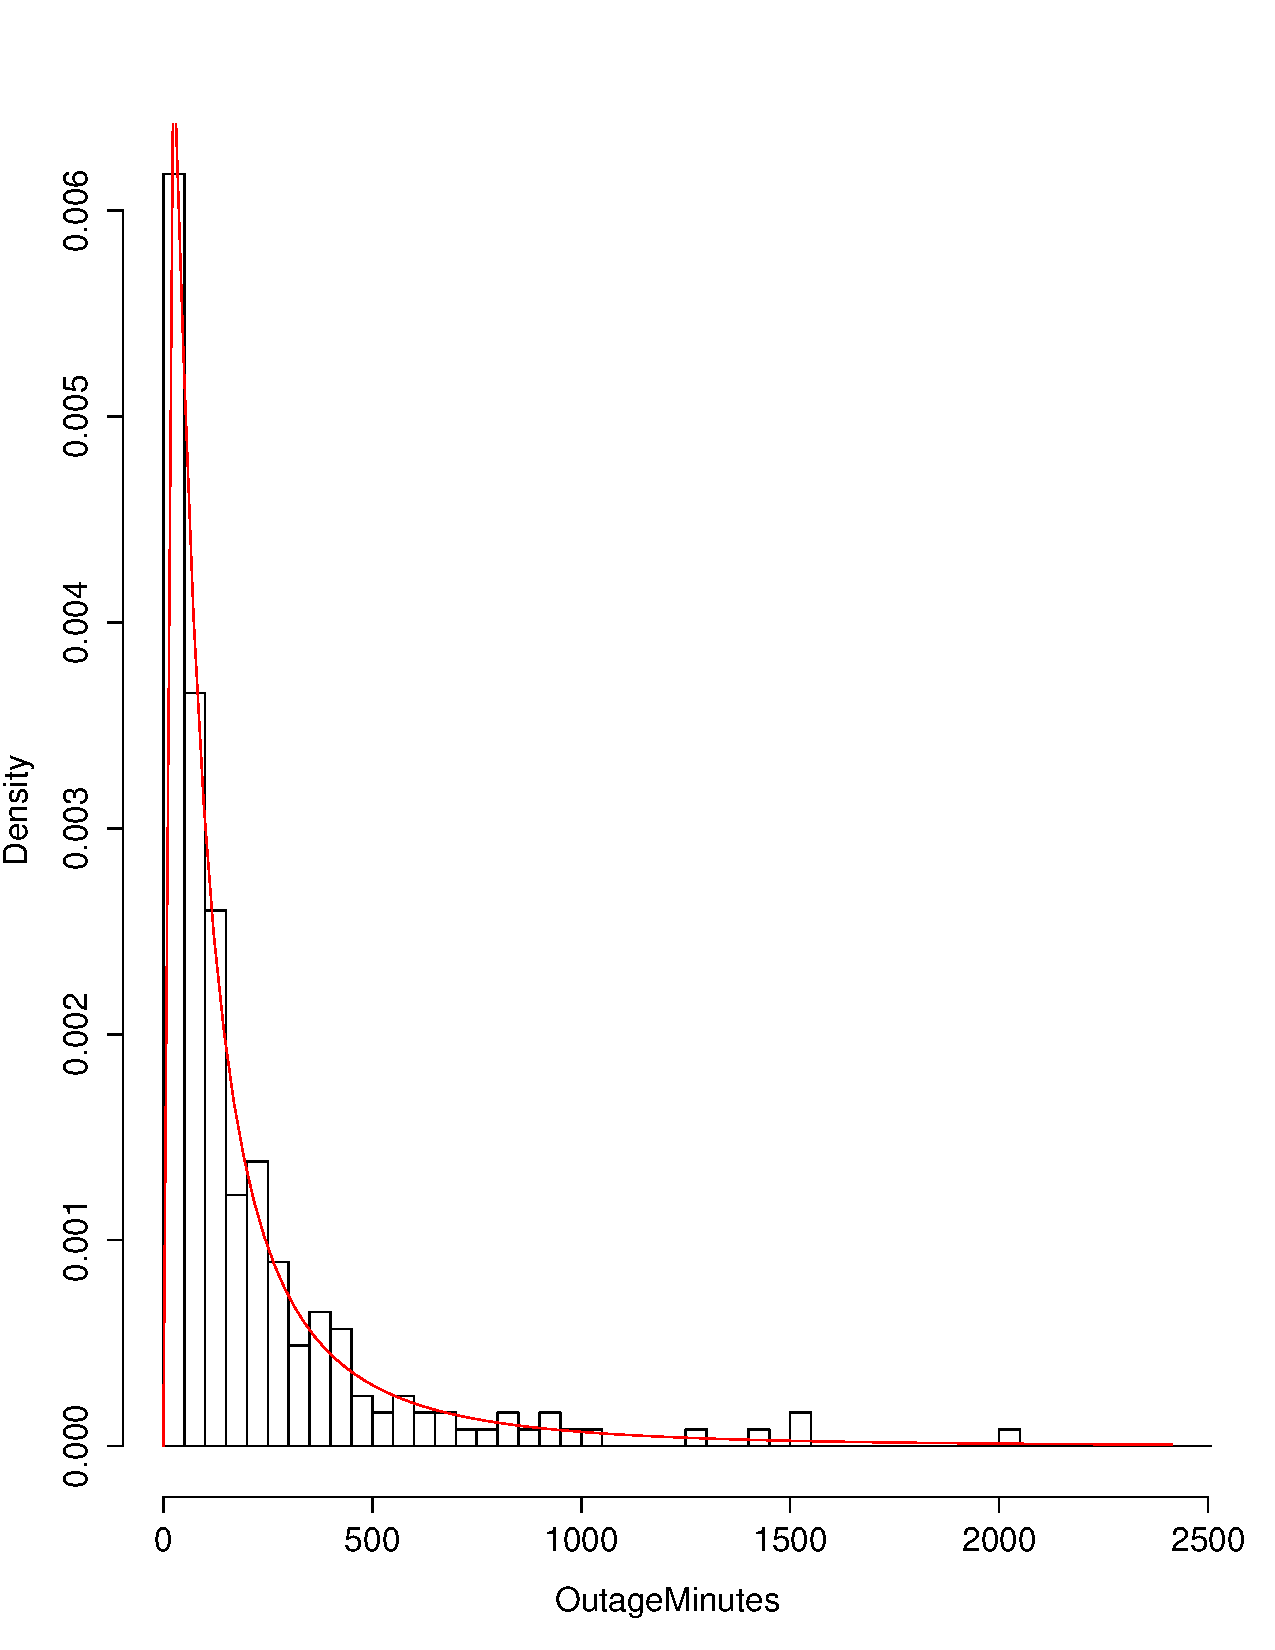
\includegraphics[width=8cm]{graph1.pdf} 
\caption{ Histogram of Outage Times (In Minutes) with fitted lognormal Curve}
\end{center}
\label{fig:outagedistribution}
\end{figure}


\begin {table}
\caption{}
%\caption {Summary statistics for all outage events}
\begin{center}
\begin{tabular}{l | r} Statistic & Value 
\\ \hline Samples & 246
\\ Mean & 314
\\ Std Dev & 1414
\\ Median & 105
\\ Skew & 13.80
\\ Distribution & lognormal
\\AD GoF Test (p) & 0.95
\end{tabular}
\end{center}
\end{table}


\subsection{Outage Component}

Table III lists the summary statistics of outage events broken down by Component. E-Mail recorded the highest proportion of all outages. BSS/social recorded had the lowest. Outages are most likely to happen in the E-mail component. \par

Due to the small number of samples (16) recorded for the BSS/social category, the goodness of fit value should be treated with caution. \par


\begin {table}
\caption {Summary statistics for outages by component with lognormal GoF} 
\begin{center}
\begin{tabular}{l | c | c | c | c} Statistic & BSS/Social & Collaboration & Email & Mixed
\\ \hline Samples & 16 & 34 & 152 & 43
\\ \% Samples & 7 & 14 & 62 & 17
\\ Mean & 274 & 189 & 258 & 626
\\ Std Dev & 639 & 379 & 423 & 3261
\\ Median & 45	& 61.5 & 126.5 & 85
\\ Skew & 3.56	& 3.83 & 5.45 & 6.30
\\AD GoF (p) & 0.69 & 0.62 & 0.99 & 0.64
\end{tabular}
\end{center}
\end{table}


\subsection{Outage Type}

Table IV lists the summary statistics of outage events broken down by type. Configuration/Manual and Contention/Concurrency recorded the highest proportion of outages while Hardware/Other had the lowest. Outages are most likely to be either Configuration/Manual or Contention/Concurrency. 

Due to the smallnumber of samples (23) for the Hardware/Other category, the goodness of fit value should be treated with caution. \par


\begin {table}
\caption {Summary statistics for outages by type with lognormal GoF} 
\begin{center}
\begin{tabular}{p{1.26cm} |  p{1.3cm} | p{1.3cm} | p{0.9cm} | p{0.9cm} | p{1cm}} Statistic & Configuration & Contention & Disaster & Network & Hardware
\\ & Manual & Concurrency &  Recovery & & Other
\\ \hline \# Samples & 74 & 64 & 36 & 49 & 23
\\ \% Samples & 30 & 26 & 15 & 20 & 9
\\ Mean & 488 & 239 & 134 & 	315	& 243
\\ Std Dev & 2488	& 469 & 161	& 591 	& 358
\\ Median & 114.5	& 86	& 72	& 145	& 91
\\ Skew & 8.28	& 3.69	& 2.33	& 5.30	& 2.11
\\AD GoF  & 0.91 & 0.97 & 0.94 & 0.75 & 0.96
\end{tabular}
\end{center}
\end{table}


\subsection{Data Centre Location}

Table V lists the summary statistics of outage events broken down by data centre. Data Centre A recorded the highest proportion of outages, while Data centre B had the lowest. The remaining 3\% were from outages found in all thee data centres.  Outages are most likely to happen within Data Centre A.

Eight outages were found in all three data centres. Due to the small number of samples detailed analysis was not performed. Furthermore the researches felt it in was inappropriate to merge these eight samples into one of the existing data centre pools as this may confound analysis and results from a single data centre category. \par

\begin {table}
\caption {Summary statistics for outages by data centre with lognormal GoF} 
\begin{center}
\begin{tabular}{l | c | c | c} Statistic & Data Centre A & Data Centre B  & Data Centre C 
\\ \hline Samples & 160 & 24 & 54 
\\ \% Samples & 65 & 10 & 22
\\ Mean & 224	& 188 	& 645
\\ Std Dev & 313	& 280 & 2961
\\ Median & 113.5	& 89.5	& 79.5
\\ Skew & 2.93	& 2.89	& 6.67 
\\AD GoF (p) & 0.99 & 0.99 & 0.31 
\end{tabular}
\end{center}
\end{table}
%\vspace{-2mm}

\section{Discussion}

Section IV provided an outline of outage events that were studied as part of our overall dataset, including distribution, component, outage type and data centre location. The following section provides deeper analysis of the results. In each section references will be made to each research question asked in section III.

\subsection{Outage Distribution}

To answer the question how are the times of cloud outage events distributed, an Anderson Darling goodness of fit test was conducted against a number of distributions; Exponential, Gamma, lognormal and Weibull. With the exception of lognormal,  the p values were very low, which indicated that these distribution types were a poor fit. For lognormal a p value was found to be 0.95. \par

In this case the hypothesis that the outage times are Log normally distributed is a surprisingly good fit. Fig. 1 and Table II clearly show that the distribution type is lognormal. This finding further expands the applicability of the use of the lognormal distribution of model repair times. It is known that repairable systems typically refer to mechanical, electric and electronic systems. However given the above results we can now include software systems as another subtype.\par

It is also worth noting that the mean outage time is approximately 314 minutes, which indicates that resolution of an outage in complex system architecture is a non-trivial task. Additionally with a standard deviation found to be approximately 1414 minutes and a skew value of 13.80, clearly indicates that there is a high level of dispersion within the dataset. \par

Given the nature of cloud computing, new code updates and configuration changes are made on a regular basis. It is not uncommon for an enterprise to introduce changes on a bi-weekly or monthly basis. Therefore with this high level of system activity it is not unsurprising that outages can occur frquently. If a state of the art outage tracking system were introduced, it would be interesting to determine overall as both process improvements were made coupled with underlying code stability to observe the overall affect on both the distribution type and shape. This would provide a concrete answer to questions such as: what impact do specific process improvements make to overall outage times? As a business where do resources need to be deployed to improve platform stability: Development, Operations or Quality Assurance? \par

\subsection{Outage Component}

Examining outages by component can give insight as to which component are likely to exhibit outages and whether these times vary by component. \par

Table III provides summary details of outages by component. It was noted that mixed components had the highest mean outage time with 627 minutes, followed by BSS/social, Mail with 274 \& 258 respectively and Collaboration with 189 minutes. Consequently mixed components also has the highest standard deviation and skew. In all cases, each component class had a good fit to a lognormal distribution, with the e-mail category fitting best with a p value of 0.99. However the BBS-Social category has a low number of samples, therefore the goodness of fit assessment should be treated with some caution. \par

Based on these results it is clear that the e-mail component has the highest proportion of outages. Tiger teams should review the root cause of each outage related to the e-mail component.  This will gain understanding as to the what types of failures contribute most to e-mail outage events. Triangulating each outage event against the failure type and data centre location can help business and operations teams resource their crisis teams on a per component basis.

Secondly the results show that mixed components have the highest mean outage time. This result seems logical, given that when an outage occurs across common infrastructure and/or multiple components that the repair time is greater. There are many systems to check and repair as part of the remediation process. To verify, the individual reports were checked for mixed component failures. It was found that one outage took multiple days to resolve. Hence skewing the overall mean time. While this data point may be considered an outlier in the classic sense, given this was a real fault, it must be included as part of analysis. Tiger teams should determine the the root cause of each outage to intersect failure type and data centre to understand common failure patterns. \par


\subsection{Outage Type}
Examining outages by type gives a deeper understanding of what types of problems are likely to cause an outage within a cloud infrastructure. Table IV provides this insight. \par

Significantly Configuration/Manual had the highest expected outage time with 489 minutes, with Network next highest with 315 minutes. Contention/Concurrency, Hardware and Disaster recovery had expected outages times of 239, 243 and 134 minutes respectively. Finally the outage times of each category were fitted with a lognormal distribution. In each case the hypothesis of whether a lognormal distribution was a suitable distribution could not be rejected. However one caveat is that the Hardware/Other category had a low number of samples, so this result must be treated with caution. \par

It is clear that issues related to Configuration/Manual contribute most to the overall number of outages but also take the longest to resolve.  Given the relative complexity of the overall cloud architecture it is apparent that a system of managed configuration changes is required. Firstly to ensure that for all configuration changes made, that there is a commit and rollback feature to ensure that that harmful (extreme) configuration settings can be reversed if required. Additionally tiger teams should implement a system, which can monitor real-time configuration changes across all data centres.  \par

With any distributed system the network health plays an important role in system stability. The network issues studied fell into two main categories: network congestion and temporary network outages. For congestion issues, business and operations teams need to define clear bandwidth capacity requirements to ensure that their infrastructure has the bandwidth to meet the demands of their existing user base and future subscription signings. The underlying application code and middleware stack should have additional resiliency added to ensure that temporary outages do not cause cascade failures.  \par

\subsection{Data Centre Location}

Table V provides summary details of outages by data centre. As discussed previously in section III, user concurrency varies by data centre. Data Centre C had the highest mean outage time with 645 minutes, while data centre's A \& B had mean outages times of 224 and 188 respectively. All three data centre outage times were modelled with a lognormal distribution and both data centre A \& B were an excellent fit. Each had a  p value of 0.99. Data centre C faired worst in terms of fit with a p value of 0.31. Even with this value the hypothesis of whether a log normal distribution is a suitable fit cannot be rejected. \par

In some ways the above results are expected, it seems intuitive that a high use data centre would incur the most outages due to the high level of customer activity, however even with all these outages the mean outage time is 224 minutes, which is approximately 90 minutes less than the overall mean. What appears somewhat counter intuitive is that data centre C has the second highest number of outages and the highest mean outage time. From closer inspection the mean outage time of data centre C is due to a small number of outages with high durations. Finally it is worth noting that Data centre B has the lowest number of outage events and the lowest mean outage time.\par

In the context of software delivery to multiple data centres, the same code is released to each system. Clearly customers are impacted in different ways depending on which data centre is used. With this knowledge, tiger teams can investigate in two areas. Firstly does the underlying customer use case of each data centre vary? Secondly a root and branch investigation of each data centre configuration should be conducted and compared for discrepancies, with specific focus on the configuration of the e-mail component. \par
%\vspace{-1mm}

\section{Conclusion}
The purpose of this study was to examine the duration of outage events within a Cloud based application platform. It was found that the lognormal distribution is a useful distribution for modelling repair times of SaaS Outages. The findings of this study support previous research particularly in the field of system reliability and repair times. \par

Previous studies have shown that shown that Cloud Outages are an infrequent occurrence. Additionally we show that the lognormal distribution is a useful tool for modelling repair times in mechanical and electronic maintainable systems. \par

This work provides a more comprehensive study in relation to how outage times can vary between failure type, component and the data centre used at the time of an outage. \par

In future SMEs can assess their outage data to understand the core issues that effect their underlying service platform. A specific operations framework can then be developed to allow SMEs to focus on specific areas of their architecture or business process, which impede reliability. Likewise, by usage of this framework on an iterative basis, an SME can then set realistic remediation targets. \par

In future work we shall assess our framework in conjunction with the time between outage events to understand how best operations teams can be deployed where parallel outage events occur.  \par
%\vspace{-2mm}

% An example of a floating figure using the graphicx package.
% Note that \label must occur AFTER (or within) \caption.
% For figures, \caption should occur after the \includegraphics.
% Note that IEEEtran v1.7 and later has special internal code that
% is designed to preserve the operation of \label within \caption
% even when the captionsoff option is in effect. However, because
% of issues like this, it may be the safest practice to put all your
% \label just after \caption rather than within \caption{}.
%
% Reminder: the "draftcls" or "draftclsnofoot", not "draft", class
% option should be used if it is desired that the figures are to be
% displayed while in draft mode.
%
%\begin{figure}[!t]
%\centering
%\includegraphics[width=2.5in]{myfigure}
% where an .eps filename suffix will be assumed under latex, 
% and a .pdf suffix will be assumed for pdflatex; or what has been declared
% via \DeclareGraphicsExtensions.
%\caption{Simulation Results}
%\label{fig_sim}
%\end{figure}

% Note that IEEE typically puts floats only at the top, even when this
% results in a large percentage of a column being occupied by floats.


% An example of a double column floating figure using two subfigures.
% (The subfig.sty package must be loaded for this to work.)
% The subfigure \label commands are set within each subfloat command, the
% \label for the overall figure must come after \caption.
% \hfil must be used as a separator to get equal spacing.
% The subfigure.sty package works much the same way, except \subfigure is
% used instead of \subfloat.
%
%\begin{figure*}[!t]
%\centerline{\subfloat[Case I]\includegraphics[width=2.5in]{subfigcase1}%
%\label{fig_first_case}}
%\hfil
%\subfloat[Case II]{\includegraphics[width=2.5in]{subfigcase2}%
%\label{fig_second_case}}}
%\caption{Simulation results}
%\label{fig_sim}
%\end{figure*}
%
% Note that often IEEE papers with subfigures do not employ subfigure
% captions (using the optional argument to \subfloat), but instead will
% reference/describe all of them (a), (b), etc., within the main caption.


% An example of a floating table. Note that, for IEEE style tables, the 
% \caption command should come BEFORE the table. Table text will default to
% \footnotesize as IEEE normally uses this smaller font for tables.
% The \label must come after \caption as always.
%
%\begin{table}[!t]
%% increase table row spacing, adjust to taste
%\renewcommand{\arraystretch}{1.3}
% if using array.sty, it might be a good idea to tweak the value of
% \extrarowheight as needed to properly center the text within the cells
%\caption{An Example of a Table}
%\label{table_example}
%\centering
%% Some packages, such as MDW tools, offer better commands for making tables
%% than the plain LaTeX2e tabular which is used here.
%\begin{tabular}{|c||c|}
%\hline
%One & Two\\
%\hline
%Three & Four\\
%\hline
%\end{tabular}
%\end{table}


% Note that IEEE does not put floats in the very first column - or typically
% anywhere on the first page for that matter. Also, in-text middle ("here")
% positioning is not used. Most IEEE journals/conferences use top floats
% exclusively. Note that, LaTeX2e, unlike IEEE journals/conferences, places
% footnotes above bottom floats. This can be corrected via the \fnbelowfloat
% command of the stfloats package.




% conference papers do not normally have an appendix


% use section* for acknowledgement
%\section*{Acknowledgment}


%The authors would like to thank...





% trigger a \newpage just before the given reference
% number - used to balance the columns on the last page
% adjust value as needed - may need to be readjusted if
% the document is modified later
%\IEEEtriggeratref{8}
% The "triggered" command can be changed if desired:
%\IEEEtriggercmd{\enlargethispage{-5in}}

% references section

% can use a bibliography generated by BibTeX as a .bbl file
% BibTeX documentation can be easily obtained at:
% http://www.ctan.org/tex-archive/biblio/bibtex/contrib/doc/
% The IEEEtran BibTeX style support page is at:
% http://www.michaelshell.org/tex/ieeetran/bibtex/

\bibliographystyle{IEEEtran}
% argument is your BibTeX string definitions and bibliography database(s)
\bibliography{served}

%
% <OR> manually copy in the resultant .bbl file
% set second argument of \begin to the number of references
% (used to reserve space for the reference number labels box)


% that's all folks
\end{document}


